\subsection{PostgreSQL Configuration}\label{subsec:postgresql-configuration}
\begin{flushleft}
    Currently, the database contains 2 databases.
    \begin{itemize}
        \item contact\_form
        \item shop
    \end{itemize}
    As a security feature, the login either by local or remote host, have enabled "SCRAM-SHA-256".
\end{flushleft}
\subsubsection[Contact database]{Contact database}
\begin{flushleft}
    As the name hints, this database is used to store the contact forms received using the contact page from the website.
    Yet, the database consists of one table.
\end{flushleft}

\begin{center}
    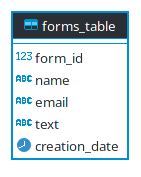
\includegraphics[scale=0.6]{DB_Table_Schema_Contact_FormV1}
\end{center}
\begin{center}
    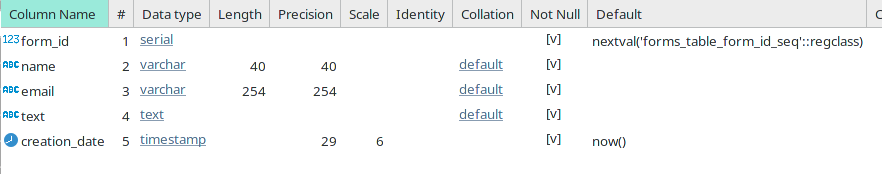
\includegraphics[scale=0.6]{DB_Table_Table_Contact_Form}
\end{center}

\begin{flushleft}
    As the name hints, this database is used to store the contact forms received using the contact page from the website.
    Yet, the database consists of one table.
\end{flushleft}
\begin{flushleft}
    It also contains a procedure called "insert\_form", which given the next information "\textit{(p\_name varchar,
    p\_email varchar, p\_text text)}", checks if the values are valid and in case of not being valid, will rise an error
    (more information in the REGEX and Error threads).
\end{flushleft}
\begin{flushleft}
    As a security measure, there been a user implemented using the next query:
    \begin{lstlisting}[language=SQL,label={lst:lstlisting}]
REVOKE ALL ON DATABASE contact_form FROM PUBLIC;
CREATE USER form_user with password 'form_pass';
GRANT CONNECT ON DATABASE contact_form to form_user;
GRANT EXECUTE on procedure insert_form to form_user;
GRANT USAGE on SEQUENCE contact_form.public.forms_table_form_id_seq to form_user;
GRANT INSERT on TABLE forms_table to form_user;
    \end{lstlisting}
\end{flushleft}
\begin{flushleft}
    Taking a look at the query, we can observe that the first step is to revoke all the permissions in the database,
    that way we can ensure that all the users are limited to the options that we specifically gave.
\end{flushleft}
